\textbf{Beskriv forskellige m\aa der at h\aa ndtere constraint, samt beskriv deres fordele og ulemper!}

- \gls{mpc} \\
- \gls{clf} combined wiht \gls{cbf} (stabilization property of CLF
with the safety aspect from the CBF)   \\
- reference governor?\\

\section{Safety Precautions for Automated Surgery Control}\label{sec:safety-def}
A crucial matter when dealing with those topics within robotic surgeries feature necessary conditions to guarantee the patient safety and to avert patient trauma \citep{bib:safety}.




The system considered will be the general non-linear system on the form:
\begin{flalign*}
\dot{x} = f(x) + g(x)\,u + h(x)\,d
\end{flalign*}
\vspace{-0.7cm}

\begin{longtable}{p{.9\textwidth} p{.1\textwidth} p{.1\textwidth}} 
where & & \\
\gls{x} is the state and restricted to $x \in \mathbb{R}^n$ where  \gls{n} is the number of states &[$\cdot$]& \\
\gls{u} is the control input and restricted to $u \in \mathbb{R}^m$ where \gls{m} is the number of inputs& [$\cdot$]& \\
\gls{d} is the disturbance input and restricted to $d \in D \subseteq \mathbb{R}^p$ where \gls{p} is the number of disturbances & [$\cdot$]& \\
\gls{f} is a potential non-linear function, $f:\mathbb{R}^n \rightarrow \mathbb{R}^n$ & [$\cdot$]& \\
\gls{g} is a potential non-linear function, $g:\mathbb{R}^n \rightarrow \mathbb{R}^{n \times m}$ & [$\cdot$]& \\
\gls{h} is a potential non-linear function, $h:\mathbb{R}^n \rightarrow \mathbb{R}^{n \times p}$ & [$\cdot$]& 
\end{longtable}

The definition of safety will follow the definition described in \citep{bib:safety}, i.e.:
\begin{exa}
A closed loop control system, $\Gamma_\text{cl} = (f_\text{cl},h,X,X_0.X_u,D)$, is unsafe if there exist a time $t \in [0,$\gls{T}$]$ such that the trajectory $\phi_{X_0}^{\bar{d}} : [0,T]$ satisfy: 
\begin{flalign}
		\left( \phi_{X_0}^{\bar{d}}([0,t]) \cap X_u \right) \neq \emptyset \kk \wedge \kk 
		\phi_{X_0}^{\bar{d}}([0,t]) \subseteq X
	\label{eq:defsafety}
\end{flalign}

The closed loop system $\Gamma_\text{cl}$ is safe if there are no unsafe trajectories.
\vspace{-0.2cm}

\begin{longtable}{p{.9\textwidth} p{.1\textwidth} p{.1\textwidth}} 
Where  & & \\
\gls{fcl} is a potential non-linear function with the closed loop characteristic:\\ \kk $f_\text{cl}: x \mapsto f(x)+g(x)k(x)$ where \gls{k} is the feedback gain with the map $k: \mathbb{R}^n \rightarrow \mathbb{R}^m$ & [$\cdot$] &  \\
\gls{X} is the set of all allowed states & [$\cdot$] &  \\
\gls{X0} is the set of all allowed initial states & [$\cdot$] &  \\
\gls{Xu} is the set of all unsafe states & [$\cdot$] &  \\
\gls{phi} is the set of all allowed initial conditions with the bounded disturbance input \gls{dbar} & [$\cdot$]
\end{longtable}

A graphical interpretation can be deduced from \autoref{eq:defsafety} and found in \autoref{fig:defsafety}.

\begin{figure}[H]
	\center
	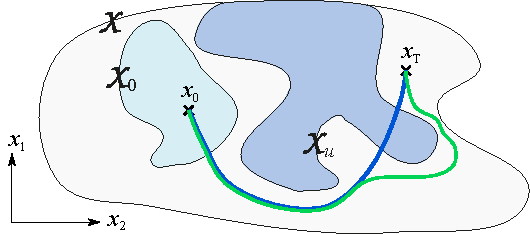
\includegraphics[width=0.75\textwidth]{safety.pdf}	
	\caption{Graphically interpretation of \autoref{eq:defsafety} in the state space. The blue trajectory is unsafe while the green trajectory is safe.}
	\label{fig:defsafety}
\end{figure}
\label{def_safety}
\end{exa}



\gls{lie}

If the system always moves very slowly, acceleration may be ignored and maybe dyamics could be ignored altogether, only leaving the evolution of kinematics in the function $f(x)$.

The design of a safe controller features the property that a supplied control signal ensures compliance of the definition described in \autoref{sec:safety-def}.

A one-dimensional simple case is analysed at first. The approach adopted constitute the movement of instrument slide, see \autoref{fig:lol}.

\begin{figure}[H]
	\center
	--- NICE FIGURE OF INSTRUMENT SLIDE ---
	\caption{nice figure}
	\label{fig:lol}
\end{figure}

A barrier certificate function can be constructed from the definitions, i.e.:
\begin{flalign}
& B(x) \leq 0 \kk  \forall \hspace{0.3cm} x \in \mathcal{X}_0  \label{cer1}\\
& B(x) > 0  \kk  \forall \hspace{0.3cm} x \in \mathcal{X}_u \label{cer2} \\
& L_f(B(x)) \leq 0 \kk  \forall \hspace{0.3cm} x \in \mathcal{X} \label{cer3}
\end{flalign}
\vspace{-0.8cm}
\begin{longtable}{p{.9\textwidth} p{.1\textwidth} p{.1\textwidth}} 
	Where  & & \\
	\gls{bar} is the barrier function & [$\cdot$] \\ 
\end{longtable}
\vspace*{-0.2cm}


